\begin{figure}[H]
    \centering
    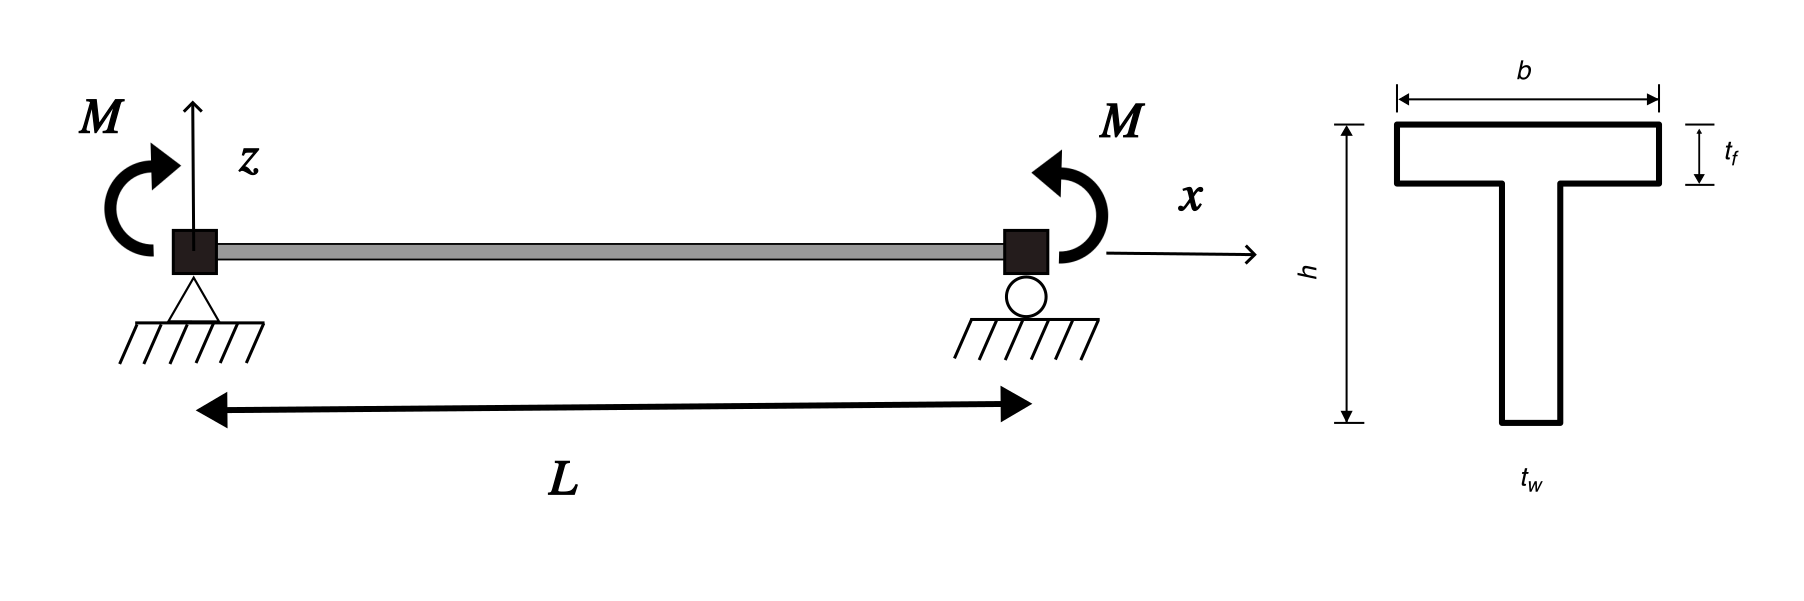
\includegraphics[width=0.7\linewidth]{Examples/frame-1035/img/frame-1035-model.png}
    \caption{Model for Example~\ref{sec:frame-1035}.}
    \label{fig:1035-model}
\end{figure}

\FrameSection{
label/problem=frame-1035,
E=200,
G=80,
unit/stress={\giga\pascal}
}

A simply supported span is subjected to constant flexure (\cref{fig:1035-model}). 
A closed form solution for the critical buckling moment is \citep{kitipornchai1986lateral}:
$$
\begin{aligned}
M_c & =\frac{\pi}{L}\sqrt{E I_y G J} \left[\left(1+\frac{\pi^2 \beta_x^2 E I_y}{4L^2 G J}\right)^{1 / 2}+\frac{\pi \beta_x}{2 L}\left(\frac{E I_y}{G J}\right)^{1 / 2}\right] .
\end{aligned}
$$

\begin{Note}
From \cite{du2021threedimensionala}:
For the section properties shown in Fig. 12, buckling loads are obtained for three different beam lengths using 20 the newly developed mixed elements. 
The comparison of the results from the present study and Kitipornchai’s theoretic equation are presented in Table 1. 
It is shown that the lateral-torsional buckling loads are accurately predicted by the mixed elements. 
In the analysis, a five-point Gauss-Lobatto integration rule is used for each element.
\end{Note}

\begin{figure}[H]
    \centering
    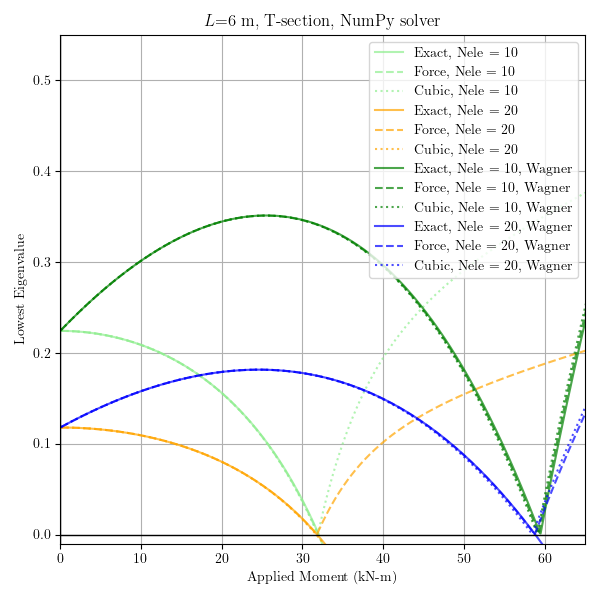
\includegraphics[width=0.5\linewidth]{Examples/frame-1035/img/Figure_5.png}
    \caption{Stiffness eigenvalues from Example~\ref{sec:frame-1035}.}
    \label{fig:1035}
\end{figure}
